\documentclass[12pt]{article}
\usepackage{graphicx}
\usepackage{caption}
\usepackage[hypcap=false]{caption}
\usepackage{geometry}
\usepackage{listings}
\usepackage{amsthm}
\geometry{margin=1in}
\RequirePackage{amsmath}
\usepackage{cite}
\usepackage{booktabs}
\usepackage{amsmath,amssymb,amsfonts,amsthm}
\usepackage{algorithmic}
\usepackage{textcomp}
\usepackage{xcolor}
\usepackage{txfonts}
\usepackage{enumitem}
\usepackage{mathtools}
\newcommand{\rupee}{\text{Rs.}}
\usepackage{gensymb}
\usepackage{comment}
\usepackage[breaklinks=true]{hyperref}
\usepackage{tkz-euclide} 
\usepackage{listings}                                                            \usepackage[utf8]{inputenc}     
\usepackage{xparse}
\usepackage{color}                                            
\usepackage{array}                                            
\usepackage{longtable}                                       
\usepackage{calc}               
\usepackage{multirow}
\usepackage{multicol}
\usepackage[version=4]{mhchem} 
\usepackage{hhline}                                           
\usepackage{ifthen} 
\usepackage{lscape}
\usepackage{tabularx}
\usepackage{array}
\usepackage{float}
\usepackage{gvv}
\usepackage{gvv-book}


\author{EE25BTECH11010-ARSH DHOKE}
\title{GATE CY 2024 questions}
\date{}

\begin{document}
\maketitle

\section*{General Aptitude (GA)}
\textbf{Q.1 -- Q.5 Carry ONE mark Each}

\begin{enumerate}
\item $\Delta G_f^\circ$ and $\Delta H_f^\circ$ for Fe(g) are $370.7~\text{kJ mol}^{-1}$ and $416.3~\text{kJ mol}^{-1}$ at 298 K, respectively. Assuming $\Delta H_f^\circ$ is constant in the interval 250 K to 375 K, $\Delta G_f^\circ$ (rounded off to the nearest integer) for Fe(g) at 375 K is:

\begin{enumerate}
\begin{multicols}{2}
\item 359 kJ mol$^{-1}$
\item 338 kJ mol$^{-1}$
\item 325 kJ mol$^{-1}$
\item 310 kJ mol$^{-1}$
\end{multicols}
\end{enumerate}
\hfill (GATE CY 2024)

\item The 15 parts of the given figure are to be painted such that no two adjacent parts with shared boundaries (excluding corners) have the same color. The minimum number of colors required is

\begin{center}
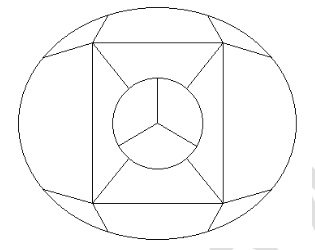
\includegraphics[width=0.4\columnwidth]{figs/q2.png}
\captionof{figure}{Figure for Q.2}
\label{fig:q2}
\end{center}

\begin{enumerate}
\begin{multicols}{2}
\item 4
\item 3
\item 5
\item 6
\end{multicols}
\end{enumerate}
\hfill (GATE CY 2024)

\item How many 4-digit positive integers divisible by 3 can be formed using only the digits \{1, 3, 4, 6, 7\}, such that no digit appears more than once in a number?

\begin{enumerate}
\begin{multicols}{2}
\item 24
\item 48
\item 72
\item 12
\end{multicols}
\end{enumerate}
\hfill (GATE CY 2024)

\item The sum of the following infinite series is

\[
2 + \frac{1}{2} + \frac{1}{3} + \frac{1}{4} + \frac{1}{8} + \frac{1}{9} + \frac{1}{16} + \frac{1}{27} + \cdots
\]

\begin{enumerate}
\begin{multicols}{2}
\item $\dfrac{11}{3}$
\item $\dfrac{7}{2}$
\item $\dfrac{13}{4}$
\item $\dfrac{9}{2}$
\end{multicols}
\end{enumerate}
\hfill (GATE CY 2024)

\item In an election, the share of valid votes received by the four candidates A, B, C, and D is represented by the pie chart shown. The total number of votes cast in the election were 1,15,000, out of which 5,000 were invalid.

\begin{center}
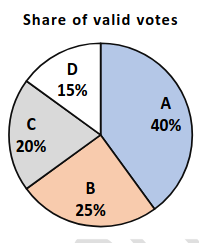
\includegraphics[width=0.45\columnwidth]{figs/q5.png}
\captionof{figure}{Figure for Q.5}
\label{fig:q5}
\end{center}

Based on the data provided, the total number of valid votes received by the candidates B and C is

\begin{enumerate}
\item 45,000
\item 49,500
\item 51,750
\item 54,000
\end{enumerate}

\hfill (GATE CY 2024)

\item Thousands of years ago, some people began dairy farming. This coincided with a number of mutations in a particular gene that resulted in these people developing the ability to digest dairy milk.

Based on the given passage, which of the following can be inferred?

\begin{enumerate}
\item All human beings can digest dairy milk.
\item No human being can digest dairy milk.
\item Digestion of dairy milk is essential for human beings.
\item In human beings, digestion of dairy milk resulted from a mutated gene.
\end{enumerate}
\hfill (GATE CY 2024)

\item The probability of a boy or a girl being born is $1/2$. For a family having only three children, what is the probability of having two girls and one boy?
\begin{multicols}{2}
\begin{enumerate}
\item $3/8$
\item $1/8$
\item $1/4$
\item $1/2$
\end{enumerate}
\end{multicols}
\hfill (GATE CY 2024)


\item Person 1 and Person 2 invest in three mutual funds A, B, and C. The amounts they invest in each of these mutual funds are given in the table.

\begin{center}
\begin{center}
\begin{tabular}{ll}
    \textbf{Group I} & \textbf{Group II} \\
    P. Ferrite & 1. Hexagonal Close Packed (HCP) \\
    Q. Austenite & 2. Body Centered Cubic (BCC) \\
    R. Martensite & 3. Body Centered Tetragonal (BCT) \\
    & 4. Face Centered Cubic (FCC)
\end{tabular}
\end{center}
 \captionsetup{type=table}
\captionof{table}{Table for Q.8}
\end{center}

At the end of one year, the total amount that Person 1 gets is \rupee500 more than Person 2. The annual rate of return for the mutual funds B and C is 15\% each. What is the annual rate of return for the mutual fund A?

\begin{enumerate}
\item 7.5\%
\item 10\%
\item 15\%
\item 20\%
\end{enumerate}
\hfill (GATE CY 2024)

\item Three different views of a dice are shown in the figure below.

\begin{center}
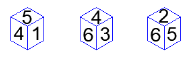
\includegraphics[width=0.35\columnwidth]{figs/q9.png}
\captionof{figure}{Figure for Q.9}
\label{fig:q9}
\end{center}

The piece of paper that can be folded to make this dice is

\begin{enumerate}
\item 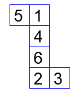
\includegraphics[width=0.25\columnwidth]{figs/q9a.png}
\captionof{figure}{Option A}
\label{fig:q9a}
\item 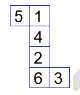
\includegraphics[width=0.25\columnwidth]{figs/q9b.png}
\captionof{figure}{Option B}
\label{fig:q9b}
\item 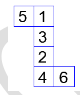
\includegraphics[width=0.25\columnwidth]{figs/q9c.png}
\captionof{figure}{Option C}
\label{fig:q9c}
\item 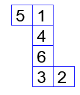
\includegraphics[width=0.25\columnwidth]{figs/q9d.png}
\captionof{figure}{Option D}
\label{fig:q9d}
\end{enumerate}
\hfill (GATE CY 2024)


\item Visualize two identical right circular cones such that one is inverted over the other and they share a common circular base. If a cutting plane passes through the vertices of the assembled cones, what shape does the outer boundary of the resulting cross-section make?

\begin{enumerate}
\item A rhombus
\item A triangle
\item An ellipse
\item A hexagon
\end{enumerate}
\hfill (GATE CY 2024)

\item Among the following, the compound with the lowest CO stretching frequency is
\begin{enumerate}
\begin{multicols}{2}
\item {[Mn(CO)$_6$]}$^+$

\item {[V(CO)$_6$]}$^-$

\item {[Cr(CO)$_5$]}

\item {[Cr(dien)(CO)$_3$]} (dien: diethylenetriamine)
\end{multicols}
\end{enumerate}
\hfill (GATE CY 2024)

\item The ground state of [Cr(H$_2$O)$_6$]$^{2+}$ is
\begin{enumerate}
\begin{multicols}{2}
\item$^5E_g$

\item$^5T_{2g}$

\item$^6A_{1g}$

\item$^6A_{2g}$
\end{multicols}
\end{enumerate}
\hfill (GATE CY 2024)

\item The reaction of XeF$_2$ with HN(SO$_2$F)$_2$ at 273 K in CF$_2$Cl$_2$ solvent yields
\begin{enumerate}
\begin{multicols}{2}
\item XeF$_4$ + SO$_2$ + NH$_3$

\item Xe + SO$_2$ + N$_2$ + HF

\item SOF$_2$ + XeO$_2$ + NH$_3$

\item FXeN(SO$_2$F)$_2$ + HF
\end{multicols}
\end{enumerate}
\hfill (GATE CY 2024)

\item The major product in the following reaction sequence is

\begin{center}
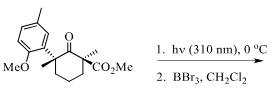
\includegraphics[width=0.35\columnwidth]{figs/q14.png}
\captionof{figure}{Figure for Q.14}
\label{fig:q14}
\end{center}
\begin{enumerate}
\item  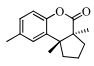
\includegraphics[width=0.24\columnwidth]{figs/q14a.png}
\captionof{figure}{Option A}
\label{fig:q14a}
\item  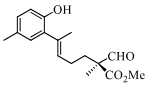
\includegraphics[width=0.24\columnwidth]{figs/q14b.png}
\captionof{figure}{Option B}
\label{fig:q14b}
\item  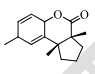
\includegraphics[width=0.24\columnwidth]{figs/q14c.png}
\captionof{figure}{Option C}
\label{fig:q14c}
\item  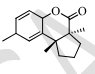
\includegraphics[width=0.24\columnwidth]{figs/q14d.png}
\captionof{figure}{Option D}
\label{fig:q14d}
\end{enumerate}
\hfill (GATE CY 2024)

\item Among the following, the chiral compound is

\begin{center}
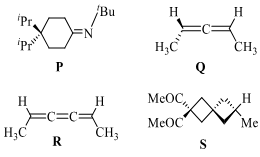
\includegraphics[width=0.5\columnwidth]{figs/q15.png}
\captionof{figure}{Figure for Q.15}
\end{center}

\begin{multicols}{2}
\begin{enumerate}
\item \textbf{P}
\item \textbf{Q}
\item \textbf{R}
\item \textbf{S}
\end{enumerate}
\end{multicols}
\hfill (GATE CY 2024)


\item The major product in the given reaction sequence is \textbf{Q}. The mass spectrum of \textbf{Q} shows

(M = molecular ion peak)

\begin{center}
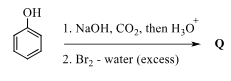
\includegraphics[width=0.35\columnwidth]{figs/q16.png}
\captionof{figure}{Figure for Q.16}
\end{center}

\begin{enumerate} 
\item M, (M+2), (M+4), and (M+6) peaks with relative intensity of 1:1:1:1
\item M, (M+2), (M+4), and (M+6) peaks with relative intensity of 1:3:3:1
\item M, (M+2), and (M+4) peaks with relative intensity of 1:2:1
\item M and (M+2) peaks with relative intensity of 1:1
\end{enumerate}
\hfill (GATE CY 2024)

\item The product M in the following reaction is

\begin{center}
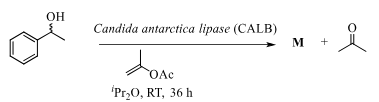
\includegraphics[width=0.45\columnwidth]{figs/q17.png}
\captionof{figure}{Figure for Q.17}
\end{center}

\begin{enumerate}
\item 
\begin{figure}[H]
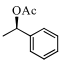
\includegraphics[width=0.1\columnwidth]{figs/q17a.png}
\captionof{figure}{Option A}
\end{figure}
\item 
\begin{figure}[H]
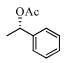
\includegraphics[width=0.1\columnwidth]{figs/q17b.png}
\captionof{figure}{Option B}
\end{figure}
\item 
\begin{figure}[H]
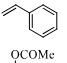
\includegraphics[width=0.1\columnwidth]{figs/q17c.png}
\captionof{figure}{Option C}
\end{figure}
\item 
\begin{figure}[H]
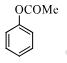
\includegraphics[width=0.1\columnwidth]{figs/q17d.png}
\captionof{figure}{Option D}
\end{figure}
\end{enumerate}
\hfill (GATE CY 2024)

\item Critical micellar concentration of a surfactant is 0.008 M in water at 25\textdegree C. If the aggregation number of the micelles is 80, the concentration of the micelles (in M) present in 0.088 M aqueous solution of the surfactant at 25\textdegree C is

\begin{enumerate}
\begin{multicols}{2}
\item 0.010
\item 0.001
\item 0.008
\item 0.088
\end{multicols}
\end{enumerate}
\hfill (GATE CY 2024)

\item The order and the number of classes present in a group with the irreducible representations A$_1$, A$_2$, B$_1$, B$_2$, E$_1$, and E$_2$ are, respectively,

\begin{enumerate}
\begin{multicols}{2}
\item 6 and 6
\item 12 and 6
\item 6 and 3
\item 12 and 3
\end{multicols}
\end{enumerate}
\hfill (GATE CY 2024)

\item The molecule XY$_2$ is microwave active and its vibration-rotation spectrum shows only P and R transitions. In the correct structure,

\begin{enumerate}
\item X is the central atom in linear XY$_2$.
\item X is the central atom in bent XY$_2$.
\item Y is the central atom in linear XY$_2$.
\item Y is the central atom in bent XY$_2$.
\end{enumerate}
\hfill (GATE CY 2024)

\item The complex(es) with distorted octahedral structure is (are)
\begin{multicols}{2}
\begin{enumerate}
\item {[VF$_6$]}$^{3-}$
\item {[FeF$_6$]}$^{3-}$
\item {[MnF$_6$]}$^{3-}$
\item {[Fe(CN)$_6$]}$^{4-}$
\end{enumerate}
\end{multicols}
\hfill (GATE CY 2024)

\item The compound(s) which show(s) the perovskite structure in solid state is (are)

\begin{enumerate}
\item CaTiO$_3$
\item NiFe$_2$O$_4$
\item Fe$_3$O$_4$
\item CsPbI$_3$
\end{enumerate}
\hfill (GATE CY 2024)

\item Among the following metalloproteins, the pair(s) of \textbf{non-heme} proteins is (are)

\begin{enumerate}
\item Hemoglobin and Myoglobin
\item Hemocyanin and Carboxypeptidase
\item Hemerythrin and Carbonic anhydrase
\item Cytochrome P-450 and Hemocyanin
\end{enumerate}
\hfill (GATE CY 2024)

\item The reaction(s) that yield(s) X as the major product is (are): 

\begin{figure}[H]
\centering
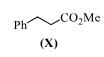
\includegraphics[width=0.4\columnwidth]{figs/q24.png}
\captionof{figure}{Figure for Q.24}
\label{fig:q24}
\end{figure}

\begin{enumerate}
\item 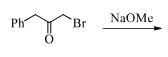
\includegraphics[width=0.4\columnwidth]{figs/q24a.png} \captionof{figure}{Option A}
\label{fig:q24a}

\item 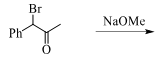
\includegraphics[width=0.4\columnwidth]{figs/q24b.png} \captionof{figure}{Option B}
\label{fig:q24b}

\item 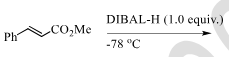
\includegraphics[width=0.4\columnwidth]{figs/q24c.png} \captionof{figure}{Option C}
\label{fig:q24c}

\item 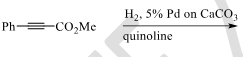
\includegraphics[width=0.4\columnwidth]{figs/q24d.png} \captionof{figure}{Option D}
\label{fig:q24d}
\end{enumerate} \hfill (GATE CY 2024)

\item The reaction(s) that yield(s) 2-methylquinoline as the major product is (are):

\begin{enumerate}
\item 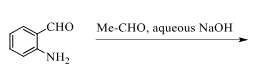
\includegraphics[width=0.45\columnwidth]{figs/q25a.png} \captionof{figure}{Option A}
\label{fig:q25a}

\item 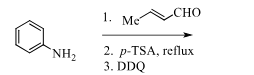
\includegraphics[width=0.45\columnwidth]{figs/q25b.png} \captionof{figure}{Option B}
\label{fig:q25b}

\item 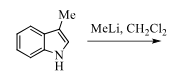
\includegraphics[width=0.45\columnwidth]{figs/q25c.png} \captionof{figure}{Option C}
\label{fig:q25c}

\item 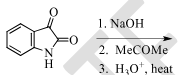
\includegraphics[width=0.45\columnwidth]{figs/q25d.png} \captionof{figure}{Option D}
\label{fig:q25d}
\end{enumerate} \hfill (GATE CY 2024)

\item The correct statement(s) for decalin is (are):

\begin{enumerate}
\item cis-Decalin is thermodynamically less stable than trans-decalin.
\item cis-Decalin contains plane of symmetry.
\item trans-Decalin undergoes ring inversion.
\item trans-Decalin belongs to the point group of C$_{2h}$.
\end{enumerate} \hfill (GATE CY 2024)

\item The correct statement(s) about $^4D_{5/2}$ state of an atom is (are):  
\begin{enumerate}
    \item it corresponds to $L = 2, S = 1/2,$ and $J = 5/2$.
    \item it can originate from $s^1p^2$ electronic configuration.
    \item it splits into five levels in the presence of magnetic field.
    \item it can show spectral transition to $^4P_{3/2}$ state.
\end{enumerate}
\hfill (GATE CY 2024)

\item The correct statement(s) related to an ensemble is (are):  
\begin{enumerate}
    \item an ensemble is a collection of an infinite number of imaginary replications of the system of interest.
    \item all members of an ensemble are macroscopically identical and also have identical microstates.
    \item an ensemble average of any macroscopic property of the system is equal to the value of the property averaged over a sufficiently long time.
    \item all systems in a canonical ensemble need NOT have the same composition.
\end{enumerate}
\hfill (GATE CY 2024)

\item The non-dissociative adsorption of a gas on a given surface at a fixed temperature follows Langmuir isotherm. The plot(s) which give(s) a straight line is (are)  
[Given: $V =$ volume of the adsorbed gas, $P =$ pressure of the gas]  
\begin{enumerate}
    \item $1/V$ versus $1/P$
    \item $P/V$ versus $P$
    \item $V$ versus $P$
    \item $V$ versus $1/P$
\end{enumerate}
\hfill (GATE CY 2024)

\item The crystal field stabilization energy of $[\text{Cr(NH}_3\text{)}_6]^{3+}$ with $\Delta_0$ value of $21600~\text{cm}^{-1}$ is $y~\text{cm}^{-1}$. The value of $|y|$ is \underline{\hspace{2cm}}.  
(rounded off to the nearest integer)  
\hfill (GATE CY 2024)

\item The number of metal-metal bond(s) in the complex $[(\eta^5\text{-Cp})\text{Mo(CO)}_2]_2$ is $x$ and in $[(\eta^5\text{-Cp})_2\text{Fe}_2(\text{CO})_3]$ is $y$. The value of $x+y$ is \underline{\hspace{2cm}}.  
(Assume 18 electron rule is followed.)  
(Answer in integer)  
\hfill (GATE CY 2024)

\item $^1\text{H}$ NMR spectrum of a mixture containing $\text{CH}_3\text{Br}$ ($x$ mol) and $(\text{CH}_3)_2\text{CBr}$ ($y$ mol) shows two singlets at 2.7 ppm and 1.8 ppm, with the relative ratio of 3:1 (integration value), respectively. The value of $x/y$ is \underline{\hspace{2cm}}.  
(rounded off to the nearest integer)  
\hfill (GATE CY 2024)

\item The value of $\dfrac{e^2}{2 \pi \varepsilon_0 a_0}$ in atomic unit of energy is \underline{\hspace{2cm}}.  
($e$: charge of electron; $a_0$: Bohr radius; $\varepsilon_0$: permittivity of vacuum)  
(rounded off to the nearest integer)  
\hfill (GATE CY 2024)

\item The partial vapor pressure of 0.1 molal solution of \textbf{B} in liquid \textbf{A} is 60 kPa at 300 K. The partial vapor pressure (in kPa) of a solution containing \textbf{B} with mole fraction of 0.1 in liquid \textbf{A} at 300 K is \underline{\hspace{2cm}}.  
(Assume the solute \textbf{B} obeys Henry’s law. The molar mass of \textbf{A} is 80 g mol$^{-1}$.)  
(rounded off to three decimal places)  
\hfill (GATE CY 2024)

\item Consider the following two parallel irreversible first-order reactions, where $k_1 = 2k_2$ at 300 K. After complete conversion of \textbf{R} at 300 K, the concentration of \textbf{P1} in the reaction mixture was 15 mol L$^{-1}$. The initial concentration of \textbf{R} (in mol L$^{-1}$) was \underline{\hspace{2cm}}.  
\begin{center}
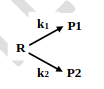
\includegraphics[width=0.35\textwidth]{figs/q35.png}
\captionof{figure}{Figure for Q.35}
\label{fig:q35}
\end{center}
($k_1$ and $k_2$ are the rate constants)  
(rounded off to one decimal place)  
\hfill (GATE CY 2024)

\textbf{Q.36 - Q.65 Carry TWO marks each.}

\item Borax on treatment with NaOH and H$_2$O$_2$ forms X. The compound X on reaction with PhCN at $60^{\circ}\mathrm{C}$ in methanol–water mixture gives Y as the major product. X and Y, respectively, are
\begin{enumerate}
\begin{multicols}{2}
  \item $\mathrm{NaB(O)(OH)_2\cdot nH_2O}$ and $\mathrm{PhCONH_2}$
  \item $\mathrm{NaB(O)(OH)_2\cdot nH_2O}$ and $\mathrm{PhCOOH}$
  \item $\mathrm{Na_2B_2(O_2)(OH)_4\cdot nH_2O}$ and $\mathrm{PhCONH_2}$
  \item $\mathrm{Na_2B_2(O_2)(OH)_4\cdot nH_2O}$ and $\mathrm{PhCOOH}$
  \end{multicols}
\end{enumerate}
\hfill (GATE CY 2024)

\item In the EPR spectrum of an aqueous solution of $\mathrm{VOSO_4}$ at room temperature, the total number of hyperfine splitting signals is
\begin{enumerate}
\begin{multicols}{2}
  \item 3
  \item 7
  \item 5
  \item 8
  \end{multicols}
\end{enumerate}
\hfill (GATE CY 2024)

\item The hapticity of allyl and Cp and the ligation mode of NO in the thermodynamically stable complexes $[(\eta^{\,x}\text{-allyl})\mathrm{Ru}(\mathrm{CO})_2(\mathrm{NO})]$ and $[(\eta^{\,y}\text{-Cp})\mathrm{Ru}(\mathrm{CO})_2(\mathrm{NO})]$, respectively, are  
(The hapticity of allyl and Cp are denoted by $\eta^{x}$ and $\eta^{y}$, respectively.)
\begin{enumerate}
  \item $(\eta^{3}, \text{NO-bent})$ and $(\eta^{5}, \text{NO-linear})$
  \item $(\eta^{3}, \text{NO-linear})$ and $(\eta^{5}, \text{NO-bent})$
  \item $(\eta^{1}, \text{NO-bent})$ and $(\eta^{3}, \text{NO-bent})$
  \item $(\eta^{1}, \text{NO-bent})$ and $(\eta^{5}, \text{NO-linear})$
\end{enumerate}
\hfill (GATE CY 2024)

\item In the following reactions, the structures of \textbf{I}, \textbf{II}, and \textbf{III}, respectively, are

\begin{center}
  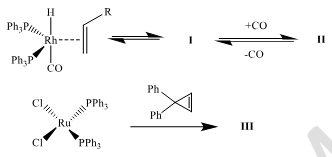
\includegraphics[width=\columnwidth]{figs/q39.png}
  
  \captionof{figure}{Figure for Q.39}
  \label{fig:q39}
\end{center}

\begin{enumerate}
  \item \begin{center}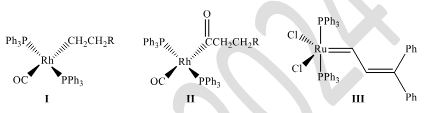
\includegraphics[width=0.6\columnwidth]{figs/q39a.png} \captionof{figure}{Option A}
  \label{fig:q39a}\end{center}
  \item \begin{center}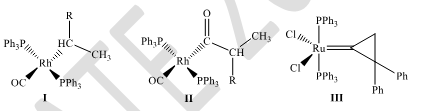
\includegraphics[width=0.6\columnwidth]{figs/q39b.png}\captionof{figure}{Option B}
  \label{fig:q39b}\end{center}
  \item \begin{center}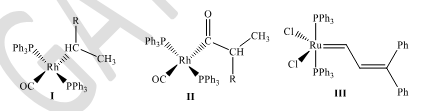
\includegraphics[width=0.6\columnwidth]{figs/q39c.png}\captionof{figure}{Option C}
  \label{fig:q39c}\end{center}
  \item \begin{center}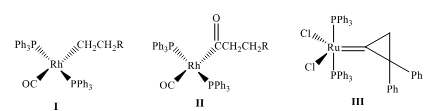
\includegraphics[width=0.6\columnwidth]{figs/q39d.png}\captionof{figure}{Option D}
  \label{fig:q39d}\end{center}
\end{enumerate}

\hfill (GATE CY 2024)

\item Consider the following $^1$H NMR (400 MHz, DMSO-d$_6$) data of a compound:

$\delta$ in ppm: 3.85 (s, 6H), 6.73 (t, $J = 2.2$ Hz, 1H), 7.1 (d, $J = 2.2$ Hz, 2H), and 13.05 (brs, 1H).

The compound is
\begin{enumerate}
\item 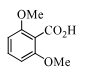
\includegraphics[width=0.5\columnwidth]{figs/q40a.png}
\captionof{figure}{Option A}
\label{fig:q40a}

\item 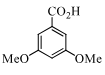
\includegraphics[width=0.5\columnwidth]{figs/q40b.png}
\captionof{figure}{Option B}
\label{fig:q40b}

\item 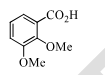
\includegraphics[width=0.5\columnwidth]{figs/q40c.png}
\captionof{figure}{Option C}
\label{fig:q40c}

\item 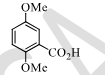
\includegraphics[width=0.5\columnwidth]{figs/q40d.png}
\captionof{figure}{Option D}
\label{fig:q40d}
\end{enumerate}
\hfill (GATE CY 2024)

\item Fischer presentation of D-\,(–)-fructose is given below.

\begin{figure}[H]
\centering
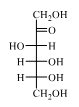
\includegraphics[width=0.35\columnwidth]{figs/q41.png}
\caption{Figure for Q.41}
\label{fig:q41}
\end{figure}

The correct structure of $\alpha$-L-(+)-fructofuranose is
\begin{enumerate}

\item 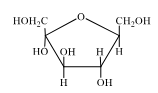
\includegraphics[width=0.45\columnwidth]{figs/q41a.png}
\captionof{figure}{Option A}
\label{fig:q41a}

\item 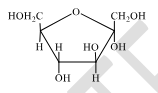
\includegraphics[width=0.45\columnwidth]{figs/q41b.png}
\captionof{figure}{Option B}
\label{fig:q41b}

\item 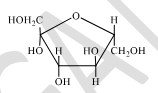
\includegraphics[width=0.45\columnwidth]{figs/q41c.png}
\captionof{figure}{Option C}
\label{fig:q41c}

\item 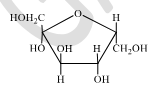
\includegraphics[width=0.45\columnwidth]{figs/q41d.png}
\captionof{figure}{Option D}
\label{fig:q41d}
\end{enumerate}
\hfill (GATE CY 2024)

\item The major products X and Y in the following reaction sequence are

\begin{figure}[H]
\centering
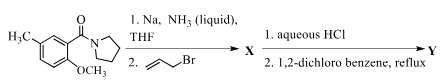
\includegraphics[width=0.7\columnwidth]{figs/q42.png}
\caption{Figure for Q.42}
\label{fig:q42}
\end{figure}

\begin{enumerate}

\item 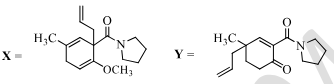
\includegraphics[width=0.45\columnwidth]{figs/q42a.png}

\captionof{figure}{Option A}
\label{fig:q42a}

\item 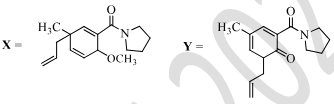
\includegraphics[width=0.45\columnwidth]{figs/q42b.png}

\captionof{figure}{Option B}
\label{fig:q42b}

\item 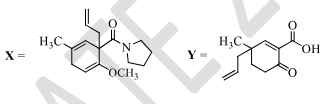
\includegraphics[width=0.45\columnwidth]{figs/q42c.png}

\captionof{figure}{Option C}
\label{fig:q42c}

\item 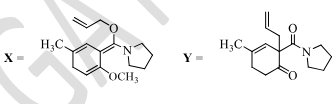
\includegraphics[width=0.45\columnwidth]{figs/q42d.png}

\captionof{figure}{Option D}
\label{fig:q42d}

\end{enumerate}
\hfill (GATE CY 2024)

\item The major products \textbf{E} and \textbf{F} in the following reaction sequence are

\begin{figure}[H]
\centering
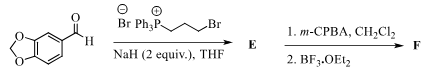
\includegraphics[width=0.7\columnwidth]{figs/q43.png}
\caption{Figure for Q.43}
\label{fig:q43}
\end{figure}

\begin{enumerate}
\item 
\begin{center}
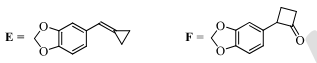
\includegraphics[width=0.5\columnwidth]{figs/q43a.png}
\captionof{figure}{Option A}
\label{fig:q43a}
\end{center}

\item 
\begin{center}
\includegraphics[width=0.5\columnwidth]{figs/q43b.png}
\captionof{figure}{Option B}
\label{fig:q43b}
\end{center}

\item 
\begin{center}
\includegraphics[width=0.5\columnwidth]{figs/q43c.png}
\captionof{figure}{Option C}
\label{fig:q43c}
\end{center}

\item 
\begin{center}
\includegraphics[width=0.5\columnwidth]{figs/q43d.png}
\captionof{figure}{Option D}
\label{fig:q43d}
\end{center}
\end{enumerate}
\hfill (GATE CY 2024)

\item $\psi_1, \psi_2, \psi_3,$ and $\psi_4$ are four Hückel molecular orbitals of benzene with orbital energies $E_1, E_2, E_3,$ and $E_4$, respectively.

\[
\psi_1 = \frac{1}{2} (\phi_B + \phi_C - \phi_E - \phi_F)
\]
\[
\psi_2 = \frac{1}{6} (\phi_A - \phi_B + \phi_C - \phi_D + \phi_E - \phi_F)
\]
\[
\psi_3 = -\frac{1}{6} (\phi_A + \phi_B + \phi_C + \phi_D + \phi_E + \phi_F)
\]
\[
\psi_4 = \frac{1}{12} (\ 2\phi_A + \phi_B - \phi_C - 2\phi_D - \phi_E + \phi_F )
\]

The correct order of the orbital energies is

(The six carbon atoms of benzene are denoted by A to F and $\phi_J$ is the 2$p_z$ orbital of $J^{th}$ carbon of benzene.)

\begin{enumerate}
\begin{multicols}{2}
\item $E_1 < E_2 = E_3 < E_4$
\item $E_4 < E_1 = E_3 < E_2$
\item $E_3 < E_1 = E_4 < E_2$
\item $E_3 < E_2 < E_1 = E_4$
\end{multicols}
\end{enumerate}
\hfill (GATE CY 2024)

\item Consider the following six vibrational modes:

\begin{quote}
symmetric stretching of CO$_2$, O-H symmetric stretching of H$_2$O, stretching of HCl, stretching of H$_2$, N-H symmetric stretching of NH$_3$, and bending of CO$_2$.
\end{quote}

Among these modes, if $k$ number of modes are IR active but Raman inactive, $l$ number of modes are IR inactive but Raman active, and $m$ number of modes are both IR and Raman active.

$k$, $l$, and $m$, respectively, are
\begin{multicols}{2}
\begin{enumerate}
\item 1, 3, and 2
\item 3, 1, and 2
\item 1, 2, and 3
\item 2, 1, and 3
\end{enumerate}
\end{multicols}
\hfill (GATE CY 2024)

\item The correct statement for a thermally initiated radical polymerization in a solution is:

\begin{quote}
(Assume: Steady-state and equal reactivity of the propagating radicals, termination reactions are only by combination, and no chain transfer reaction.
Given: Rp = rate of polymerization, DP = degree of polymerization, [I] = initiator concentration, and [M] = monomer concentration.)
\end{quote}

\begin{enumerate}
\item with increase in [I], both Rp and DP increase.
\item with increase in [M], both Rp and DP increase.
\item Rp decreases with increase in [I] but DP increases with increase in [M].
\item DP increases with increase in [I] and DP decreases with increase in [M].
\end{enumerate}

\hfill (GATE CY 2024)

\item If $q_t$ and $Q_{t,m}$ are the molecular and molar translational partition functions of X$_2$, respectively, then $\ln(Q_{t,m}) =$

\begin{quote}
(N is the Avogadro number)
\end{quote}

\begin{multicols}{2}
\begin{enumerate}
\item $N \ln q_t - N \ln N$

\item $N \ln q_t - \ln N$

\item $N \ln q_t + \ln N + N$

\item $N \ln q_t - \ln N + N$
\end{enumerate}
\end{multicols}
\hfill (GATE CY 2024)

\item Among the following, the NMR active nucleus(nuclei) is (are)

\begin{enumerate}
\begin{multicols}{2}
\item $^{12}\mathrm{C}$
\item $^{19}\mathrm{F}$
\item $^{2}\mathrm{H}$
\item $^{16}\mathrm{O}$
\end{multicols}
\end{enumerate}
\hfill (GATE CY 2024)

\item The complex(es) that exhibit(s) optical isomerism is (are)

\begin{enumerate}
\begin{multicols}{2}
\item {[Fe(acac)]}$_3$
\item \textit{cis}-{[Co(en)$_2$Cl$_2$]}$^+$
\item \textit{trans}-{[Co(en)$_2$Cl$_2$]}$^+$
\item {[Co(en)$_3$]}$^{3+}$
\end{multicols}
\end{enumerate}
\hfill (GATE CY 2024)

\item In aqueous solution of K$_4$[Fe(CN)$_6$], the allowed transition(s) is (are)
\begin{enumerate}
\begin{multicols}{2}
\item t $ ^5T_{2g} \text{ to } ^3E_g $ 

\item  $ ^1A_{1g} \text{ to } ^1T_{1g} $ 

\item  $ ^1A_{1g} \text{ to } ^1T_{2g} $ 

\item  $ ^5T_{2g} \text{ to } ^5E_g $
\end{multicols}
\end{enumerate}
\hfill (GATE CY 2024)

\item The correct option(s) that give(s) \textbf{P} as the major product is (are)

\begin{figure}[H]
\centering
\includegraphics[width=0.24\columnwidth]{figs/q51.png}
\caption{Figure for Q.51}
\label{fig:q51}
\end{figure}
\begin{enumerate}
\begin{figure}[H]
\centering
\item \includegraphics[width=0.45\columnwidth]{figs/q51a.png}
\captionof{figure}{Option A}
\label{fig:q51a}
\end{figure}

\begin{figure}[H]
\centering
\item \includegraphics[width=0.45\columnwidth]{figs/q51b.png}
\captionof{figure}{Option B}
\label{fig:q51b}
\end{figure}

\begin{figure}[H]
\centering
\item \includegraphics[width=0.45\columnwidth]{figs/q51c.png}
\captionof{figure}{Option C}
\label{fig:q51c}
\end{figure}

\begin{figure}[H]
\centering
\item \includegraphics[width=0.45\columnwidth]{figs/q51d.png}
\captionof{figure}{Option D}
\label{fig:q51d}
\end{figure}
\end{enumerate}
\hfill (GATE CY 2024)

\item The correct statement(s) regarding \textbf{P}, \textbf{Q}, \textbf{R}, and \textbf{S} is (are):

\begin{figure}[H]
\centering
\includegraphics[width=0.65\columnwidth]{figs/q52.png}
\caption{Figure for Q.52}
\label{fig:q52}
\end{figure}

\begin{enumerate}
\item \textbf{P} reacts faster than \textbf{Q} with PhSNa in DMF as a solvent.

\item \textbf{Q} reacts faster than \textbf{P} with NaN$_3$ in DMF as a solvent.

\item \textbf{R} reacts faster than \textbf{S} when treated with TsCl/Et$_3$N in DCM as a solvent.

\item \textbf{R} gets oxidized faster than \textbf{S} when reacted with CrO$_3$ in DCM as a solvent.
\end{enumerate}
\hfill (GATE CY 2024)

\item Consider the following reaction sequence. The correct option(s) is (are):

\begin{figure}[H]
\centering
\includegraphics[width=0.55\columnwidth]{figs/q53.png}
\caption{Figure for Q.53}
\label{fig:q53}
\end{figure}

\begin{enumerate}
\item \includegraphics[width=0.52\columnwidth]{figs/q53a.png} 
\captionof{figure}{Option A}
\label{fig:q53a}

\item \includegraphics[width=0.52\columnwidth]{figs/q53b.png} 
\captionof{figure}{Option B}
\label{fig:q53b}

\item \includegraphics[width=0.52\columnwidth]{figs/q53c.png} 
\captionof{figure}{Option C}
\label{fig:q53c}

\item \textbf{X} = LiAlH4; \textbf{L} = (vinylsulfonyl)benzene
\end{enumerate}

\hfill (GATE CY 2024)

\item Consider the following reaction sequence where \textbf{M} and \textbf{N} are the major products.

\begin{figure}[H]
\centering
\includegraphics[width=0.65\columnwidth]{figs/q54.png}
\caption{Figure for Q.54}
\label{fig:q54}
\end{figure}

The correct option(s) is (are):

\begin{enumerate}
\item
\begin{center}
\includegraphics[width=0.48\columnwidth]{figs/q54a.png}
\captionof{figure}{Option A}
\label{fig:q54a}
\end{center}

\item
\begin{center}
\includegraphics[width=0.48\columnwidth]{figs/q54b.png}
\captionof{figure}{Option B}
\label{fig:q54b}
\end{center}

\item
\begin{center}
\includegraphics[width=0.48\columnwidth]{figs/q54c.png}
\captionof{figure}{Option C}
\label{fig:q54c}
\end{center}

\item
\begin{center}
\includegraphics[width=0.48\columnwidth]{figs/q54d.png}
\captionof{figure}{Option D}
\label{fig:q54d}
\end{center}
\end{enumerate}
\hfill (GATE CY 2024)

\item The correct statement(s) about the relationship for the H-atoms in the following compounds is (are):

\begin{figure}[H]
\centering
\includegraphics[width=0.50\columnwidth]{figs/q55.png}
\caption{Figure for Q.55}
\label{fig:q55}
\end{figure}

\begin{enumerate}
\item H$_1$ and H$_3$ are enantiotopic; H$_2$ and H$_3$ are diastereotopic.
\item H$_1$ and H$_3$ are diastereotopic; H$_2$ and H$_3$ are enantiotopic.
\item H$_5$ and H$_7$ are enantiotopic; H$_6$ and H$_7$ are homotopic.
\item H$_5$ and H$_7$ are homotopic; H$_6$ and H$_7$ are enantiotopic.
\end{enumerate}
\hfill (GATE CY 2024)

\item Among the following, the correct statement(s) is (are):

\begin{enumerate}
\item the normalization factor of a Slater determinant for a 3-electron atom is $\sqrt{\frac{1}{3}}$.
\item the number of nodes in the radial wave function of 3s orbital of a hydrogen atom is the same as the number of nodes in the angular wave function of a 4d orbital of hydrogen atom.
\item the energy separation between any two adjacent states is same for a harmonic oscillator, while it is different for a rigid rotor.
\item the magnitude of the total spin angular momentum of an $\alpha$ electron is the negative of that of a $\beta$ electron.
\end{enumerate}
\hfill (GATE CY 2024)

\item Among the following, the correct statement(s) is (are):

\begin{enumerate}
\item C$_2$ symmetry element is present in H$_2$O and H$_2$O$_2$ but NOT in PCl$_5$.
\item both C$_2$ and C$_3$ symmetry elements are present in CCl$_4$ and SF$_6$.
\item one $\sigma_h$ and three $\sigma_d$ symmetry elements are present in benzene.
\item $\sigma_v$ symmetry element is present in NH$_3$ but NOT in BF$_3$.
\end{enumerate}
\hfill (GATE CY 2024)

\item $\Delta S^\circ$ (in J mol$^{-1}$ K$^{-1}$) for the given reaction at 298 K is \underline{\hspace{2cm}}.

\[
\ce{[Cu(H2O)6]^{2+} + en <=> [Cu(H2O)2(en)]^{2+} + 2H2O}
\]

(Given: log $K_1$ = 10.6, where $K_1$ is the equilibrium constant. $\Delta H^\circ$ = $-54$ kJ mol$^{-1}$ and R = $8.314$ J mol$^{-1}$ K$^{-1}$)
 (rounded off to two decimal places)
\hfill (GATE CY 2024)

\item The turnover frequency (in h$^{-1}$) of a reaction where 5 mol\% of a catalyst is required for 90\% conversion in 3 h is \underline{\hspace{2cm}}.
 (rounded off to the nearest integer)
\hfill (GATE CY 2024)

\item In thermogravimetric analysis, 12.45 mg of CuSO$_4\cdot$5H$_2$O was subjected to heating under N$_2$ atmosphere. At a particular temperature, there was a weight loss of 3.6 mg. The number of water molecule(s) lost per formula unit is \underline{\hspace{2cm}}.

(Given: molar mass (in g mol$^{-1}$) of H = 1.0, O = 16.0, S = 32.0, and Cu = 63.5)
 (rounded off to the nearest integer)
\hfill (GATE CY 2024)

\item In the given reaction sequence, the amount of \textbf{R} produced (in g) is \underline{\hspace{2cm}}.
\begin{figure}[H]
\centering
\includegraphics[width=0.6\columnwidth]{figs/q61.png}
\caption{Figure for Q.61}
\label{fig:q61}
\end{figure}
(Given: molar mass (in g mol$^{-1}$) of H = 1, C = 12, N = 14, O = 16, and S = 32)
(rounded off to two decimal places)
\hfill (GATE CY 2024)

\item The wave function of a particle in a cubic box (of side $L$) is given by

\[
\psi(x, y, z) = \sqrt{32}/L^3 \sin\left(\frac{\pi x}{L}\right) \cos\left(\frac{\pi x}{L}\right) \sin\left(\frac{2\pi y}{L}\right) \sin\left(\frac{\pi z}{L}\right)
\]

The ratio of the energy of the state corresponding to the above wave function to the ground state energy is \underline{\hspace{2cm}}.

(rounded off to the nearest integer)

\hfill (GATE CY 2024)


\item $\phi_1$ and $\phi_2$ are normalized eigenfunctions of a Hermitian operator.

$|\psi\rangle = 3i\;|\phi_1\rangle + 2\;|\phi_2\rangle$ and $|x\rangle = -2i\;|\phi_1\rangle + 5\;|\phi_2\rangle$.

The value of $\langle \psi | x \rangle + \langle x | \psi \rangle$ is \underline{\hspace{2cm}}.

(rounded off to the nearest integer)

\hfill (GATE CY 2024)

\item 2 mol of a monoatomic ideal gas with initial volume of 5 L and pressure 10 bar undergoes an irreversible adiabatic expansion against a constant final pressure of 1 bar. The final volume (in L) is \underline{\hspace{2cm}}.

(Given: R = $8.314 \times 10^{2}$ L bar mol$^{-1}$ K$^{-1}$)

(rounded off to one decimal place)

\hfill (GATE CY 2024)

\item The following figure shows an experimental liquid-liquid phase diagram of phenol and water at the vapor pressure of the system. The total amount of phenol and water (in mol) present in the phenol-rich phase when 5 mol of water was shaken with 5 mol of phenol at 40$^{\circ}$C is \underline{\hspace{2cm}}.

\begin{figure}[H]
\centering
\includegraphics[width=0.45\columnwidth]{figs/q65.png}
\caption{Phase diagram for Q.65}
\label{fig:q65}
\end{figure}

(rounded off to one decimal place)

\hfill (GATE CY 2024)



\end{enumerate}
\end{document}